\documentclass[11pt,letterpaper]{article}
\usepackage[lmargin=1in,rmargin=1in,tmargin=1in,bmargin=1in]{geometry}
\usepackage{../style/homework}
\usepackage{../style/commands}
\setbool{quotetype}{false} % True: Side; False: Under
\setbool{hideans}{true} % Student: True; Instructor: False

% -------------------
% Content
% -------------------
\begin{document}

\homework{7: Due 10/08}{I'm pretty but tough, like a diamond or beef jerky in a ball gown.}{Titus Andromedon, Unbreakable Kimmy Schmidt}

% Problem 1
\problem{10} Two functions $f(x)$ and $g(x)$ are plotted below. Are $f(x)$ and $g(x)$ functions? Explain. Do the functions $f(x)$ and $g(x)$ have an inverse? Explain.  
	\[
	\fbox{
	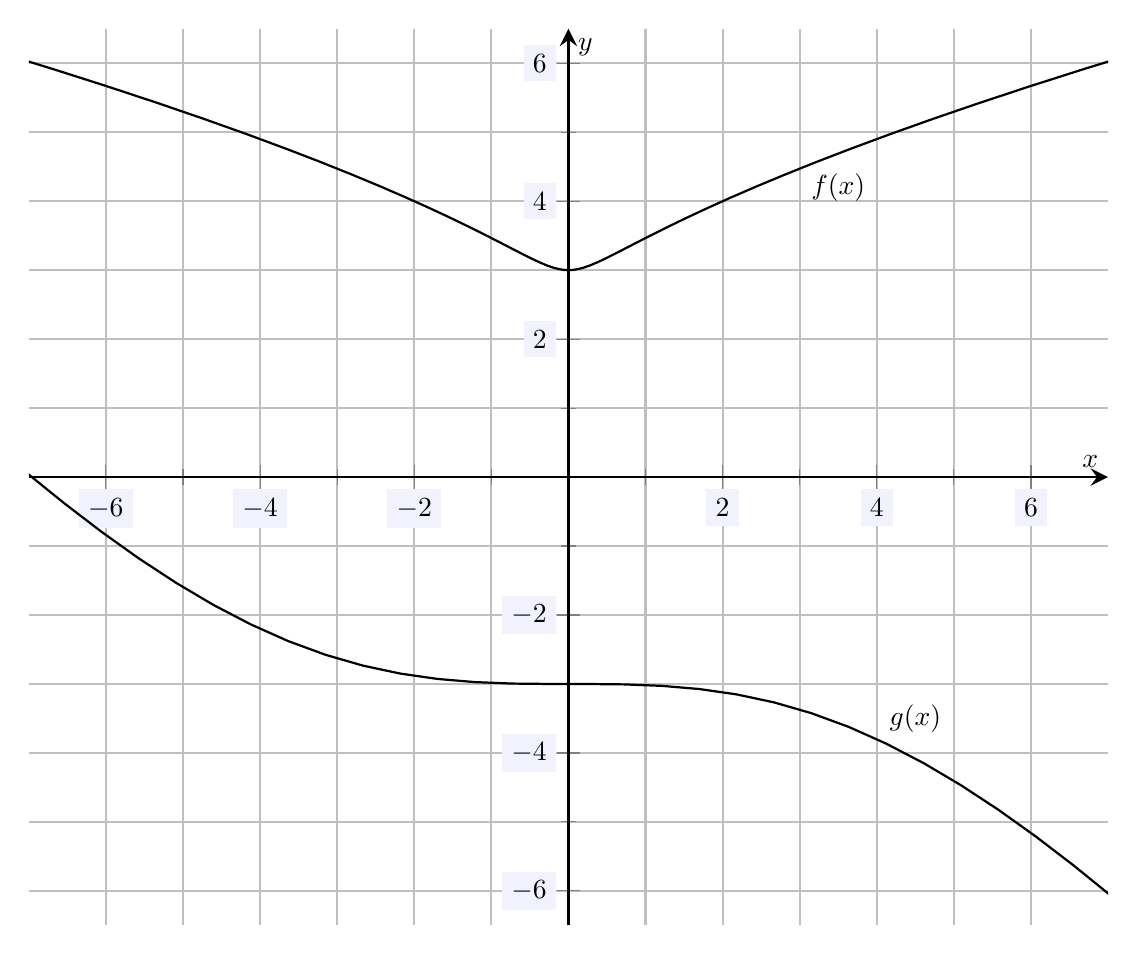
\begin{tikzpicture}[scale=2,every node/.style={scale=0.5}]
	\begin{axis}[
	grid=both,
	axis lines=middle,
	ticklabel style={fill=blue!5!white},
	xmin= -7, xmax=7,
	ymin= -6.5, ymax=6.5,
	xtick={-6,-4,-2,0,2,4,6},
	ytick={-6,-4,-2,0,2,4,6},
	minor tick = {-5,-3,...,5},
	xlabel=\(x\),ylabel=\(y\),
	]
	\node at (3.5,4.2) {$f(x)$};
	\addplot [domain= -3:3,samples=80] ({x^3 + x},{x^2 + 3}); 
	\node at (4.5,-3.5) {$g(x)$};
	\addplot [domain= -3:3,samples=100] ({8*x)},{-8*x^3/(x^2+1) - 3}); 
	\end{axis}
	\end{tikzpicture}
	}
	\]





\newpage





% Problem 2
\problem{10} Let $f(x)= 6x - 5$ and $g(x)= 2x^2 + 3x - 5$. 
	\begin{enumerate}[(a)]
	\item What is $g(2)$? 
	\item Assuming $g^{-1}$ exists, what is $g^{-1}(9)$?
	\item Assuming $f^{-1}$ exists, what is $f^{-1}(4)$?
	\end{enumerate}





\newpage





% Problem 3
\problem{10} Do the points $(1, 3)$, $(3, 7)$, and $(5,1)$ lie along a line? Justify your answer. 





\newpage





% Problem 4
\problem{10} Let $\ell(x)$ be the line through the points $(-2, 11)$ and $(3, -4)$.
	\begin{enumerate}[(a)]
	\item Find the slope of the line given by $\ell(x)$.
	\item Find the equation for $\ell(x)$.
	\item What is the $y$-intercept for $\ell(x)$?
	\item What is $\ell(-1)$?
	\end{enumerate}





\newpage





% Problem 5
\problem{10} Let $\ell(x)$ be the line through the point $(1, 3)$ with slope $\frac{1}{2}$.
	\begin{enumerate}[(a)]
	\item Find the equation for $\ell(x)$. 
	\item What is $\ell(4)$?
	\item Find the $x$-intercept for $\ell(x)$. 
	\end{enumerate}





\newpage





% Problem 6 
\problem{10} Determine if the following pairs of lines are parallel, perpendicular, or neither.
	\begin{enumerate}[(a)]
	\item $y= 5x$, \enskip $\frac{1}{5}x + y= 8$
	\item $x - 3y= 12$, \enskip $y= x + 7$
	\item $y= 3x - 1$, \enskip $6x - 2y= 4$
	\end{enumerate}





\newpage





% Problem 7
\problem{10} Find the equation of the line passing through the point $(1, -1)$ that is perpendicular to the line $y= \frac{1}{3} x - 8$. 





\newpage





% Problem 8
\problem{10} Let $f(x)= 2x - 1$. Find $f^{-1}(x)$. Show that $f^{-1}(x)$ is the inverse by showing $f(f^{-1}(x))= x$ and $f^{-1}(f(x))= x$. 





\newpage





% Problem 9
\problem{10} A cable internet company offers a high-speed internet package that costs \$62 per month, plus an additional \$85 installation fee. 
	\begin{enumerate}[(a)]
	\item Find a function that represents the total cost of purchasing internet from this company after $n$ months. 
	\item What does the $y$-intercept for this function represent?
	\item Find the total cost of the internet after 14 months.
	\item How many months of internet can you get for \$500?
	\end{enumerate}


%\printpoints
\end{document}